\subsection{Conclusions}
\paragraph{Time is slowed down near mass}
In special relativity
$$dt^2+dr^2-r^2d\Phi^2 = dt^2-dx^2-dy^2$$

Near spherical mass in general relativity proper time of body at coordinate $r$ is:
$$d\tau^2 = \left( 1- \frac{2GM}{c^2r} \right)dt^2  - \frac{dr^2}{1- \frac{2GM}{c^2r} } - r^2d\phi^2$$

where $t$,$r$,$\phi$ are time, radial distance and angle of far observer.

To calculate $r$ we take circumference of circle divided by $2\pi$. 

For body in rest time is progresses slower as body is deeper in potential well
$$d\tau = \sqrt{ 1- \frac{2GM}{c^2r} }dt$$

When $r = \frac{2GM}{c^2}$ which is called Schwarzschild radius, denominator becomes 0, and then time stops.

\paragraph{Difference of radius is more the difference of circumferences divided by $2\pi$}
Radial distance which is measured by body in rest is given by
$$ds^2 = \frac{dr^2}{ 1- \frac{2GM}{c^2r}}$$

Then measured distance between $r$ and $r+dr$ is
$$ds = \frac{dr}{\sqrt{ 1- \frac{2GM}{c^2r} }} > dr$$

It's curved geometry (not Euclidean).

\paragraph{Light is affected by gravity} Light is attracted to mass even though it's massless. Effect of gravitational lensing is based no this.
\paragraph{Light is slowed down in gravitational according to distant observer}
Local observer will still measure $c$.
\paragraph{Gravitational Doppler effect}
Light which is sent to farther radius is experiences redshift.
\paragraph{Schwarzschild radius} $R_s = \frac{2GM}{c^2}$ is event radius. No information can get outside.

$$R_s \cong 3 \left( \frac{M}{M_{\odot}} \right)km$$

\paragraph{Black hole} Mass which is concentrated inside Schwarzschild radius is a black hole which is characterized by mass, angular momentum and charge.
\paragraph{Distant observer sees fall in black hole taking infinite time} Body is stopped on Schwarzschild radius asymptotically.
\paragraph{Circular orbit of light} exist unique non-stable orbit $r = \frac{3}{2}R_s$ in which light is rotating around black hole.
\paragraph{Elliptic orbit precession}

\begin{center}
	\includegraphics[width=0.5\linewidth]{./lect26/pic1.png}
\end{center}
Effective potential in general relativity is different:
\begin{center}
	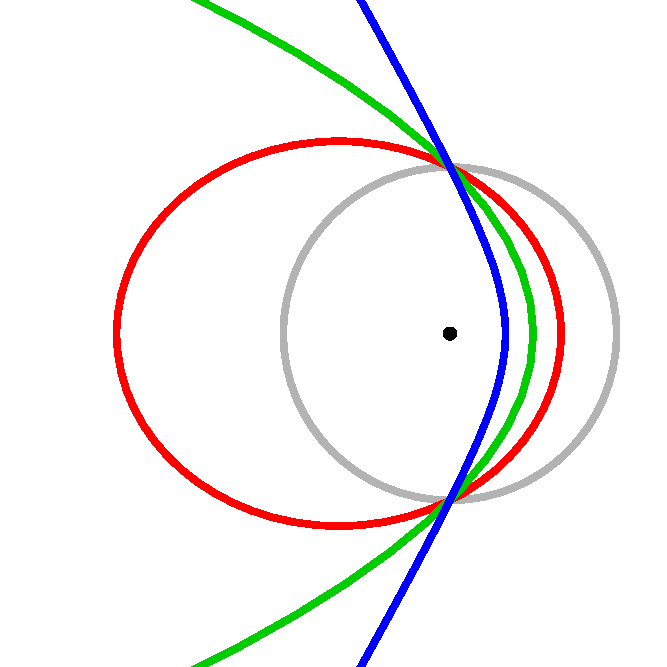
\includegraphics[width=0.5\linewidth]{./lect26/pic2.png}
\end{center}

Results are:

\begin{enumerate}
	\item There are to circular orbits: one stable (Newtonian) and one more unstable.
	\item There is no stable orbit on distance less then $r= 6\frac{GM}{c^2}$
	\item Angular cycle time is less then radial cycle time:
	
	$$ T_{r} = \frac{2\pi a^{\frac{3}{2}}}{\sqrt{GM}}\left(1 + \frac{3}{2}\frac{GM}{c^2 a} + \dots\right)  = T_{Newton}\left(1 + \frac{3}{2}\frac{v_{Kepler}^2}{c^2} + \dots\right) $$
	$$T_{\theta} = \frac{2\pi a^{\frac{3}{2}}}{\sqrt{GM}}\left(1- \frac{3}{2}\frac{GM}{c^2 a} + \dots\right) = T_{Newton}\left(1- \frac{3}{2}\frac{v_{Kepler}^2}{c^2} + \dots\right) < T_{r}$$
\end{enumerate}
\paragraph{Around rotating mass even bodies without angular momentum rotate} it is called rotational frame-dragging, since mass is dragging spacetime.
\paragraph{It is possible that body falls into black hole and it will lose mass} if the body has significant angular momentum in opposite direction.
